%% Elsevier journal template (elsarticle)
%% Target journals: Journal of Manufacturing Processes / Measurement / NDT&E International
\documentclass[preprint,12pt]{elsarticle}

\usepackage{graphicx}
\graphicspath{{../}}
\usepackage{booktabs}
\usepackage{amsmath}
\usepackage{amssymb}
\usepackage{multirow}
\usepackage{array}
\usepackage[hidelinks]{hyperref}
\usepackage{lineno}
\modulolinenumbers[5]
\setlength{\emergencystretch}{3em}

\journal{Journal of Manufacturing Processes}

\begin{document}

\begin{frontmatter}

\title{Thermal-field complexity rather than peak temperature governs porosity in laser engineered net shaping: a protocol-aware evaluation on a public Ti--6Al--4V dataset}

\author[a]{First Author\corref{cor1}}
\ead{first.author@university.edu.cn}
\author[a]{Second Author}
\author[b]{Third Author}

\cortext[cor1]{Corresponding author.}

\affiliation[a]{organization={School of Mechanical Engineering, XX University},
            addressline={XX Road},
            city={XX},
            postcode={000000},
            country={China}}

\affiliation[b]{organization={State Key Laboratory of XX},
            city={XX},
            country={China}}

\begin{abstract}
In-process pyrometry is an attractive route to porosity monitoring in laser directed energy deposition, and recent studies on public datasets report accuracies above 0.98. The reported gains, however, are obtained under random cross-validation, a protocol that lets a model exploit process position through proxies such as layer index and elapsed time. Using the public LENS Ti--6Al--4V thin-wall dataset (1564 pyrometer frames, 71 pore frames, 60 layers), we show that evaluation protocol rather than model choice determines the conclusions drawn. The four strongest tabular classifiers span only 0.03 PR-AUC under grouped cross-validation, and under forward chaining the two best are statistically indistinguishable ($p = 0.80$). We then introduce three physically interpretable thermal-field complexity descriptors---temperature histogram entropy and two gradient-magnitude statistics---that measure spatial heterogeneity of the melt pool rather than its peak value. Under forward-chaining evaluation, which trains on layers $1\!-\!k$ and tests on $k\!+\!1$ to $k\!+\!10$, the descriptors raise PR-AUC from 0.903 to 0.970 for CatBoost across ten seeds and seven split boundaries (paired $\Delta$PR-AUC $=+0.068$, 95\% CI $[0.050, 0.086]$) and reduce fold-to-fold standard deviation by 65\%. Permuted versions of the descriptors gain only 0.017, and generic distribution moments capture part of the signal but remain significantly worse (+0.028, $p<0.0001$), so the effect is specific to the information these descriptors encode rather than to dimensionality. The gain persists and grows when the two substrate-interface layers that contain 59\% of all pore frames are removed (+0.132 for XGBoost). Under the random-split protocol used in prior work the same descriptors offer no advantage (F1 0.872 versus 0.895 for a reimplementation of the published summary-statistic baseline). The value of complexity descriptors is therefore protocol-conditional: they carry transferable physics that interpolation-based evaluation systematically hides. SHAP analysis locates the risk at low entropy, low variance and high gradient, a signature consistent with under-energised, flat yet steep-edged melt pools. Cost-sensitive and abstention analyses translate these results into an operating point at which 90\% of frames are decided automatically with zero misses.
\end{abstract}

\begin{highlights}
\item Evaluation protocol changes conclusions on this dataset more than model choice does (top pair $p=0.80$).
\item Three thermal-field complexity descriptors raise forward-chained PR-AUC from 0.903 to 0.970.
\item Gains persist after removing the two substrate-interface layers holding 59\% of pore frames.
\item The descriptors help only under extrapolation; under random splits they do not.
\item SHAP links porosity to low entropy and high gradients, i.e.\ under-energised melt pools.
\end{highlights}

\begin{keyword}
Laser engineered net shaping \sep Directed energy deposition \sep Porosity prediction \sep Thermal imaging \sep Interpretable machine learning \sep Evaluation protocol
\end{keyword}

\end{frontmatter}

\linenumbers

\section{Introduction}

Laser engineered net shaping (LENS) and, more broadly, laser-based directed energy deposition (DED) build metal components by feeding powder into a moving melt pool. The process is attractive for repair and for near-net-shape production of titanium alloys, but its thermal history is sensitive to small disturbances, and lack-of-fusion pores form when the deposited energy is locally insufficient to remelt the previously deposited layer. Because porosity is interior, it is normally quantified only after fabrication by X-ray computed tomography (XCT), which is slow and cannot inform the build.

In-process pyrometry offers a way out. A dual-wavelength pyrometer views the melt pool from above at frame rates of a few hertz, and the resulting temperature field carries information about energy input, melt-pool geometry and instability. A body of work has therefore trained classifiers to map thermal measurements to porosity labels obtained from XCT \cite{khanzadeh2018,tian2020,guo2023}. Reported performance is high: recall of 98.4\% for a supervised classifier on thermal history \cite{khanzadeh2018}, and 100\% accuracy for a decision-level fusion of pyrometer and infrared networks \cite{tian2020}.

These numbers are encouraging, but they were obtained on private datasets and, in most cases, under random cross-validation. Two properties of DED thermal data make random validation optimistic. First, consecutive frames are acquired 0.15\,s apart while the deposition head advances a few millimetres, so neighbouring frames describe nearly the same melt-pool state. Second, frame index, elapsed time and layer number are available as features and correlate strongly with position in the build; a model can use them as proxies for the region of the part it is looking at. When the test set is drawn at random from the same build, such proxies remain valid and hide the model's inability to transfer.

The recent release of a thermal--porosity characterisation dataset for a LENS Ti--6Al--4V thin wall \cite{zamiela2023} makes these questions testable in public. The dataset pairs 1564 cropped pyrometer frames with XCT-derived binary pore labels registered to melt-pool coordinates. A first machine-learning study on it compared supervised and unsupervised detectors under a random 70/30 split with SMOTE \cite{ayyildizli2025}, reporting an F1 of 0.88 for a convolutional network.

This paper asks a different question: what happens when the evaluation respects the build order, and which features survive that change? Our contributions are:

\begin{enumerate}
\item We quantify how evaluation protocol shapes conclusions on this dataset. Accuracy stays between 0.972 and 0.991 across three protocols and is therefore uninformative, whereas PR-AUC and even the ranking of six classifiers change materially.
\item We introduce three thermal-field complexity descriptors---histogram entropy and two gradient-magnitude statistics---and show that they carry most of the achievable gain: three dimensions recover 96\% of the improvement obtained with a 21-dimensional spatial feature set.
\item We demonstrate that the descriptors help under forward-chaining and not under interpolation, and we explain the asymmetry: they encode transferable physics, whereas positional proxies do not.
\item We connect the statistical result to a physical mechanism through SHAP analysis, and translate it into cost-sensitive operating points and an abstention policy that reaches zero misses at 90\% automatic coverage.
\end{enumerate}

\section{Related work}

\subsection{Thermal monitoring of DED}

Melt-pool monitoring in DED has relied on coaxial or off-axis cameras, pyrometers and, more recently, hyperspectral and acoustic sensing. Khanzadeh et al.\ \cite{khanzadeh2018} established that simple descriptors of the melt pool---length, width, peak temperature, area---classify porosity poorly, and proposed morphology-based feature extraction instead, reaching a recall of 98.4\% with decision trees, $k$-nearest neighbours, support vector machines and discriminant analysis. The same group later fused pyrometer images processed by a convolutional network with infrared sequences processed by a long-term recurrent convolutional network at the decision level, and reported perfect accuracy on a Ti--6Al--4V thin wall \cite{tian2020}. Transfer of such models to new geometries was explored with a knowledge-transfer scheme that labels thermal signatures of cylinders using statistics learned on a thin wall \cite{guo2023}; the study is qualitative and reports no quantitative error.

\subsection{Machine learning for porosity prediction}

Recent work has moved toward deeper architectures and toward smaller labelled budgets. Vision transformers pretrained with a masked autoencoder have been fine-tuned on a few hundred labelled melt-pool images \cite{era2025}. Surface porosity in hybrid DED has been predicted by fusing acoustic emission with thermal imaging, with the authors noting that thermal imagery alone offers insufficient signal-to-noise ratio for small pores \cite{farea2025}. Physics-informed multimodal networks that combine melt-pool images with descriptors such as area, eccentricity, layer number and maximum temperature have been paired with SHAP-based explanations \cite{gawade2025}.

On the public dataset used here, the only published machine-learning study to our knowledge compares random forests, gradient boosting and a convolutional network against autoencoders and DBSCAN under a random 70/30 split with SMOTE, reporting an F1 of 0.88 for the network \cite{ayyildizli2025}.

\subsection{Evaluation practice}

The gap we address is methodological. Reviews of machine learning for DED quality control identify generalisation across geometries and parts as the principal open problem, and note that most studies validate ex situ and on a single build. At the same time, reported metrics are dominated by accuracy and F1 computed on random splits, which is known to be optimistic for highly imbalanced problems where accuracy is insensitive \cite{saito2015}. Conformal prediction provides distribution-free coverage guarantees and has begun to appear in additive manufacturing reliability studies, but comparative evidence in real-time monitoring remains scarce \cite{angelopoulos2023}.

\section{Data and problem formulation}

\subsection{Dataset}

We use the public dataset of Zamiela et al.\ \cite{zamiela2023} (Harvard Dataverse, DOI 10.7910/DVN/BWHYEH). A Ti--6Al--4V thin wall of 60 layers was built on an OPTOMEC LENS 750 system. A Stratonics dual-wavelength pyrometer recorded top-down melt-pool images as CSV arrays; each frame is a $200\times201$ grid of temperatures in $^\circ$C, cropped to centre the melt pool. Internal porosity was measured by a Nikon XT H225 XCT system, and pores between 0.05 and 1.00\,mm were registered to melt-pool coordinates within 0.5\,mm.

The released table contains 1564 frames with timestamps, melt-pool coordinates, area, eccentricity, peak temperature and peak location, together with a binary pore label and pore size. There are 71 pore frames (4.5\%) and 1493 pore-free frames. The build spans 457\,s. Table~\ref{tab:data} summarises the data and Fig.~\ref{fig:data} shows representative frames and the label distribution.

\begin{table}[t]
\centering
\small\setlength{\tabcolsep}{4pt}
\caption{Summary of the dataset \cite{zamiela2023}.}
\label{tab:data}
\begin{tabular}{ll}
\toprule
Property & Value \\
\midrule
Material / process & Ti--6Al--4V, LENS 750 \\
Layers & 60 \\
Frames & 1564 ($200\times201$ pixels) \\
Pore frames & 71 (4.5\%) \\
Frame interval & $\approx 0.15$\,s (6.67\,fps) \\
Temperature range & 0--1875\,$^\circ$C \\
Pore size & 0.05--0.98\,mm (median 0.33\,mm) \\
Pore frames in layers 1--2 & 42 of 71 (59.2\%) \\
\bottomrule
\end{tabular}
\end{table}

\begin{figure}[t]
\centering
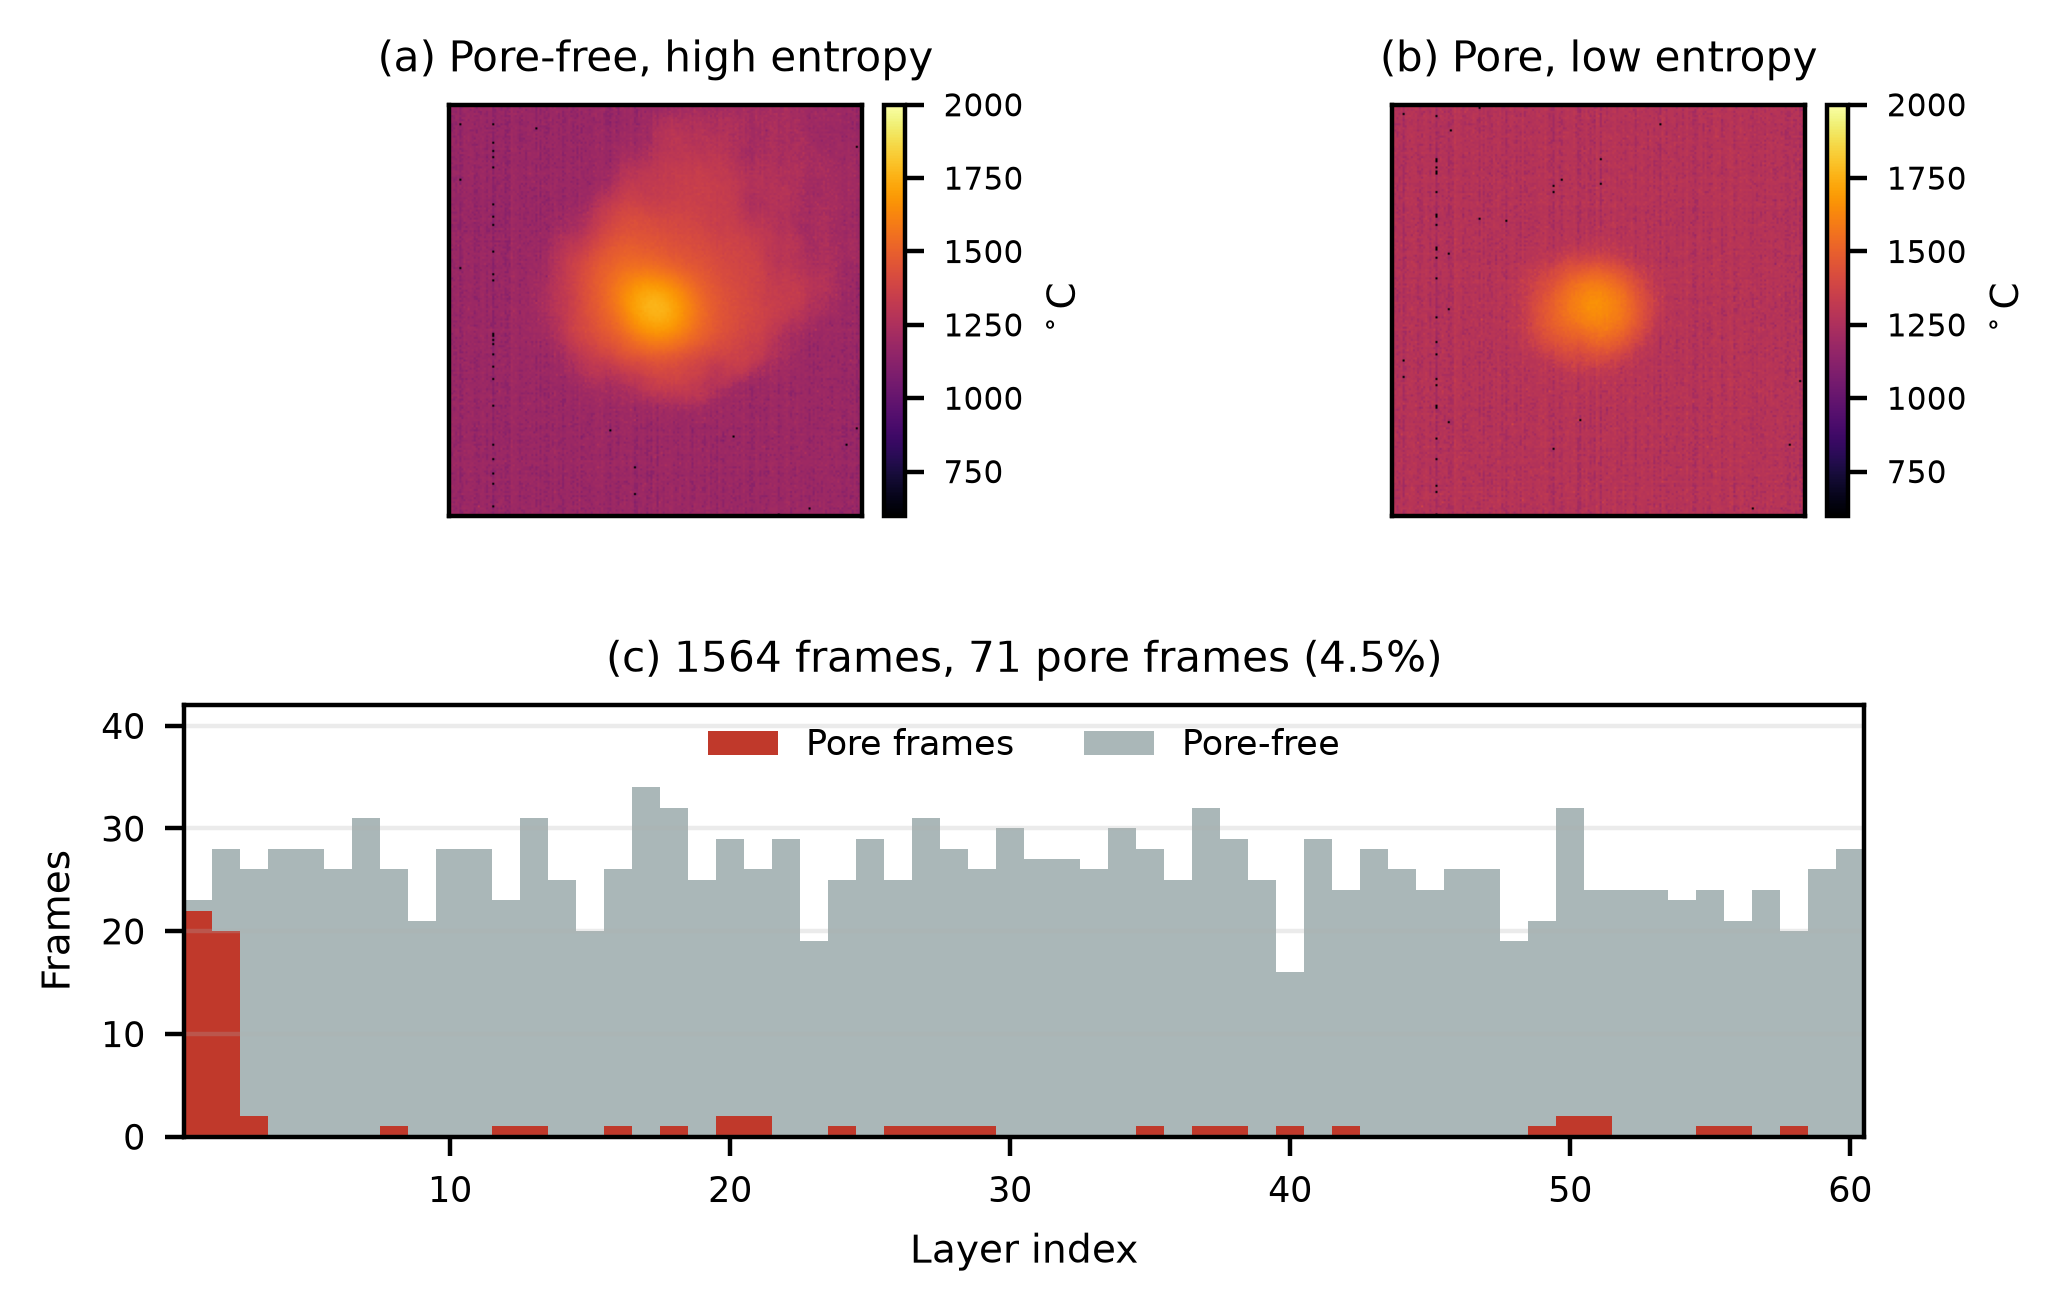
\includegraphics[width=\linewidth]{figures/fig1_dataset.png}
\caption{(a) A pore-free frame from a high-entropy region and (b) a pore-labelled frame from a low-entropy region, both displayed on the same temperature scale. (c) Distribution of frames and pore labels across the 60 layers; 59\% of pore frames occur in the first two layers, adjacent to the substrate.}
\label{fig:data}
\end{figure}

\subsection{Class imbalance and its spatial structure}

The positive rate of 4.5\% means that a trivial classifier labelling every frame as pore-free achieves 95.5\% accuracy. More importantly, the positives are not spread evenly through the build: 42 of 71 occur in layers 1 and 2, where the melt pool interacts with the substrate and lack-of-fusion is expected. A rule that labels layers 1 and 2 as positive attains a PR-AUC of 0.506 and an ROC-AUC of 0.793 without inspecting any thermal data. Any model evaluated on the full build can therefore benefit from this artefact, and we treat it explicitly in Section~\ref{sec:robust}.

\subsection{Task}

We formulate frame-level binary classification: given the features extracted from frame $t$ and its metadata, predict whether the XCT label at that location is positive. Frame-level labels are the natural unit here because the pyrometer samples faster than the layer is completed; a layer-level variant is reported in Section~\ref{sec:robust}.

\section{Method}

\subsection{Baseline features}

The baseline feature set (18 dimensions) reproduces what a practitioner would compute from the released table and the raw frame:

\begin{itemize}
\item process and position: elapsed time, $Y$, $Z$, melt-pool area, melt-pool eccentricity, peak temperature;
\item global temperature statistics: mean, standard deviation, median, 95th and 99th percentiles;
\item hot-area fractions above 800, 1200 and 1500\,$^\circ$C;
\item geometry of the hot region above 1500\,$^\circ$C: centroid row and column, and the two spatial standard deviations.
\end{itemize}

These features describe the magnitude of the thermal signal. They do not describe its spatial structure.

\subsection{Thermal-field complexity descriptors}

We add three descriptors computed directly from the temperature field $T(r,c)$ in each frame:

\paragraph{Histogram entropy}
\begin{equation}
H = -\sum_{b} p_b \log p_b ,
\end{equation}
where $p_b$ is the fraction of pixels in the $b$-th of 32 bins spanning 0--2000\,$^\circ$C. Entropy is high when the frame contains a broad range of temperatures and low when the field is dominated by a narrow band, as happens when the melt pool is shallow and the surrounding metal remains close to a uniform temperature.

\paragraph{Mean gradient magnitude}
\begin{equation}
G_{\mathrm{mean}} = \frac{1}{|\Omega_r|}\sum_{\Omega_r}|\partial_r T| \;+\; \frac{1}{|\Omega_c|}\sum_{\Omega_c}|\partial_c T|,
\end{equation}
i.e.\ the sum of the mean absolute row-wise and column-wise forward differences over the frame, with $\Omega_r$ and $\Omega_c$ the corresponding pixel sets.

\paragraph{99th percentile of gradient magnitude}
$G_{99}$ captures the steepest interfaces present in the field, complementing the mean.

The three descriptors are scale-free with respect to the absolute temperature level: they respond to the shape of the distribution and to spatial variation. Their physical reading is that a melt pool receiving insufficient energy is flat across its interior while remaining sharply bounded, whereas a well-formed pool has a broad, smoothly varying high-temperature zone.

\subsection{Models}

We evaluate logistic regression, random forest \cite{breiman2001}, XGBoost \cite{chen2016}, LightGBM, CatBoost \cite{prokhorenkova2018}, TabPFN \cite{hollmann2025}, a compact convolutional network operating on downsampled temperature fields ($67\times67$), and a one-class SVM trained on pore-free frames only. All implementations use scikit-learn \cite{pedregosa2011} or the respective official packages. Hyperparameters were fixed a priori except where noted, so that differences between feature sets are not confounded with tuning.

\subsection{Evaluation protocols}

\paragraph{Grouped cross-validation (interpolation)} Five folds formed by partitioning the 60 layers; all frames of a layer fall in the same fold. This prevents leakage between temporally adjacent frames but still allows the model to interpolate between seen process states.

\paragraph{Forward chaining (extrapolation)} The model is trained on layers $1$ to $k$ and tested on layers $k+1$ to $k+10$. We use $k\in\{20,30,40,50\}$ for the main comparison and $k\in\{15,20,\dots,45\}$ for the stability analysis. This mimics deployment, where the model is fitted on completed builds or earlier portions of a build and applied to material deposited later.

\paragraph{Random split (literature protocol)} A stratified 70/30 split with SMOTE applied to the training portion, repeated ten times, reproducing \cite{ayyildizli2025}.

\subsection{Metrics and statistical testing}

Because positives are rare, we report the area under the precision--recall curve (PR-AUC) as the primary metric, with ROC-AUC and accuracy as secondary \cite{saito2015}. Operating points are reported at a false-positive rate of 5\% on the negative class and at cost-sensitive thresholds chosen on out-of-fold predictions within the training portion.

Uncertainty is assessed in two ways. A \emph{split-level} paired bootstrap resamples the thirty (ten seeds, three protocols) test splits and tests whether the gain is consistently positive across splits. A \emph{layer-level} bootstrap resamples whole layers and tests whether the gain transfers to unseen layers. The two address different questions and are reported separately.

\section{Results}

\subsection{Baselines and the effect of protocol}

Table~\ref{tab:baseline} reports six classifiers and two deep/one-class baselines on the 18-dimensional baseline features. Under grouped cross-validation the models cluster between 0.84 and 0.94 PR-AUC; under forward chaining the spread widens and the ranking changes. CatBoost is the best model under grouping (0.938) and fourth under forward chaining (0.845), whereas TabPFN moves from joint third to first. The convolutional network, which sees the raw field, is the weakest supervised model once its stopping epoch is chosen on held-out validation layers: $0.777 \pm 0.065$ under grouping and $0.688 \pm 0.172$ under forward chaining. Its fold-to-fold spread is also the largest of any supervised model in Table~\ref{tab:baseline}.

\begin{table}[t]
\centering
\small\setlength{\tabcolsep}{4pt}
\caption{Baseline results on the 18-dimensional feature set. Mean $\pm$ standard deviation over folds or over the four forward-chaining splits. OC-SVM is trained on pore-free frames only, with kernel hyperparameters selected on the training fold. The CNN stops at the epoch that maximises PR-AUC on validation layers held out from the training portion; the test fold is never used for model selection.}
\label{tab:baseline}
\begin{tabular}{lcc}
\toprule
Model & Grouped CV (PR-AUC) & Forward chaining (PR-AUC) \\
\midrule
Logistic regression      & $0.907 \pm 0.094$ & $0.716 \pm 0.196$ \\
Random forest            & $0.840 \pm 0.037$ & $0.777 \pm 0.139$ \\
XGBoost                  & $0.910 \pm 0.067$ & $0.871 \pm 0.083$ \\
LightGBM                 & $0.912 \pm 0.095$ & $0.855 \pm 0.124$ \\
CatBoost                 & $\mathbf{0.938 \pm 0.058}$ & $0.845 \pm 0.131$ \\
TabPFN                   & $0.910 \pm 0.087$ & $\mathbf{0.901 \pm 0.128}$ \\
\midrule
CNN ($67\times67$ field) & $0.777 \pm 0.065$ & $0.688 \pm 0.172$ \\
OC-SVM (semi-sup.)& $0.759 \pm 0.089$ & -- \\
\bottomrule
\end{tabular}
\end{table}

The difference between the two strongest models under forward chaining is not significant: a paired bootstrap over test frames gives $\Delta$PR-AUC $=+0.018$ (TabPFN relative to XGBoost) with a 95\% interval of $[-0.102, +0.140]$ and $p=0.80$. Model selection, in other words, offers little on this dataset.

Accuracy tells a different and misleading story (Fig.~\ref{fig:protocol}b). It lies between 0.972 and 0.991 under all three protocols, including the random split, and therefore cannot distinguish a model that generalises from one that memorises position. PR-AUC, by contrast, moves by up to 0.09 between protocols.

\begin{figure}[t]
\centering
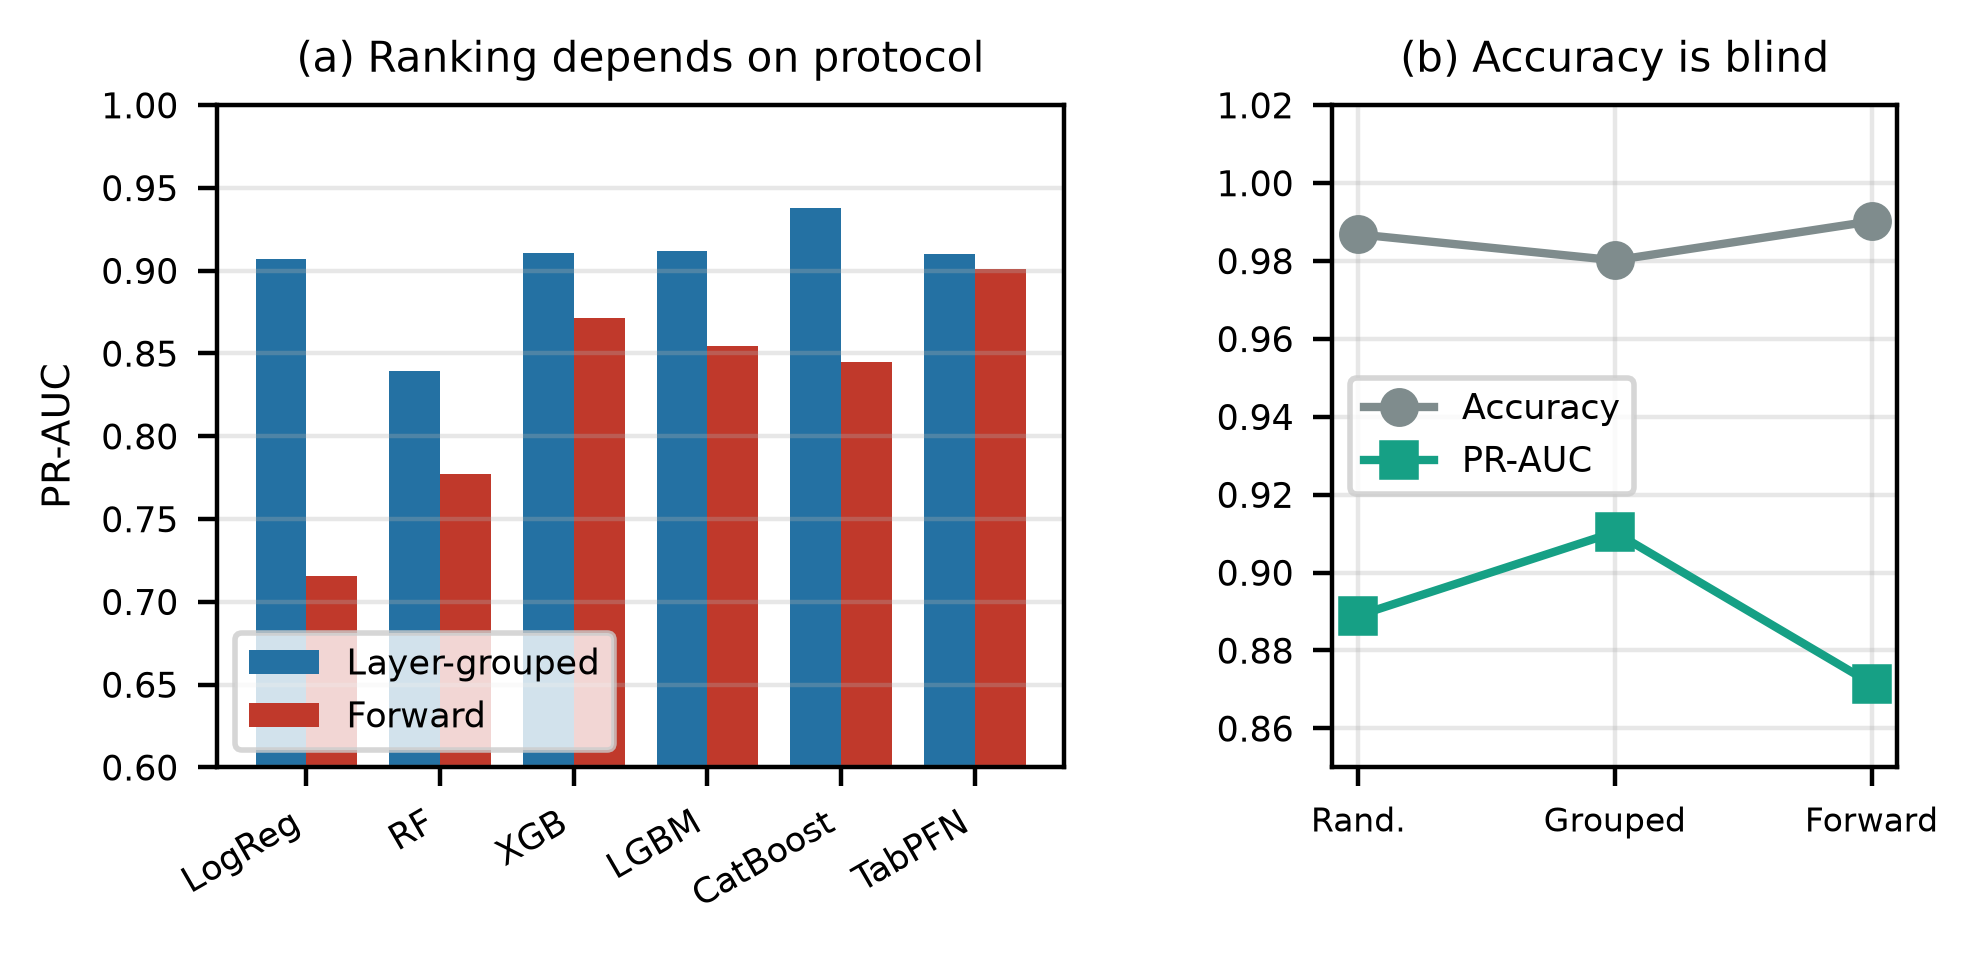
\includegraphics[width=\linewidth]{figures/fig2_protocol.png}
\caption{(a) PR-AUC of six classifiers under grouped cross-validation and forward chaining; the ranking changes with the protocol. (b) Accuracy is nearly constant across random, grouped and forward-chaining splits, whereas PR-AUC varies.}
\label{fig:protocol}
\end{figure}

\subsection{Feature ablation}

Adding the three complexity descriptors to the baseline raises forward-chained PR-AUC for CatBoost from 0.845 to 0.952, while adding the remaining 18 spatial descriptors on top yields only 0.956 (Table~\ref{tab:combo}, Fig.~\ref{fig:ablation}a). The three descriptors thus recover 96\% of the total improvement available from the full 39-dimensional set.

\begin{table}[t]
\centering
\small\setlength{\tabcolsep}{4pt}
\caption{Feature combinations. CatBoost, forward chaining ($k=20,30,40,50$) and grouped CV.}
\label{tab:combo}
\begin{tabular}{lccc}
\toprule
Feature set & Dim. & Forward chaining & Grouped CV \\
\midrule
Baseline                       & 18 & $0.845 \pm 0.131$ & $0.938$ \\
Baseline + entropy             & 19 & $0.933 \pm 0.051$ & $0.936$ \\
Baseline + gradient            & 20 & $0.912 \pm 0.041$ & $0.940$ \\
Baseline + entropy + gradient  & 21 & $\mathbf{0.952 \pm 0.047}$ & $\mathbf{0.955}$ \\
Baseline + entropy + gradient + area & 25 & $0.949 \pm 0.045$ & $0.955$ \\
Full spatial set               & 39 & $0.956 \pm 0.015$ & $0.941$ \\
\bottomrule
\end{tabular}
\end{table}

A group-wise ablation clarifies where the gain comes from (Table~\ref{tab:groups}, Fig.~\ref{fig:ablation}b). Entropy alone contributes $+0.088$ and the gradient statistics $+0.067$ under forward chaining. Hot-spot topology (12 descriptors of connected components) and Moran's $I$ contribute little, and topology actually degrades grouped performance by 0.058. We therefore retain only the three descriptors.

\begin{table}[t]
\centering
\small\setlength{\tabcolsep}{4pt}
\caption{Group-wise ablation. Each group is added to the baseline separately; values are PR-AUC for CatBoost.}
\label{tab:groups}
\begin{tabular}{lcccc}
\toprule
Group & Dim. & Forward & $\Delta$ forward & $\Delta$ grouped \\
\midrule
Entropy                        & 1  & 0.933 & $+0.088$ & $-0.001$ \\
Gradient statistics            & 2  & 0.912 & $+0.067$ & $+0.002$ \\
Hot-spot topology              & 12 & 0.899 & $+0.054$ & $-0.058$ \\
Multi-threshold area           & 4  & 0.891 & $+0.046$ & $+0.014$ \\
Moran's $I$ and peak offset    & 2  & 0.857 & $+0.012$ & $-0.019$ \\
\bottomrule
\end{tabular}
\end{table}

\begin{figure}[t]
\centering
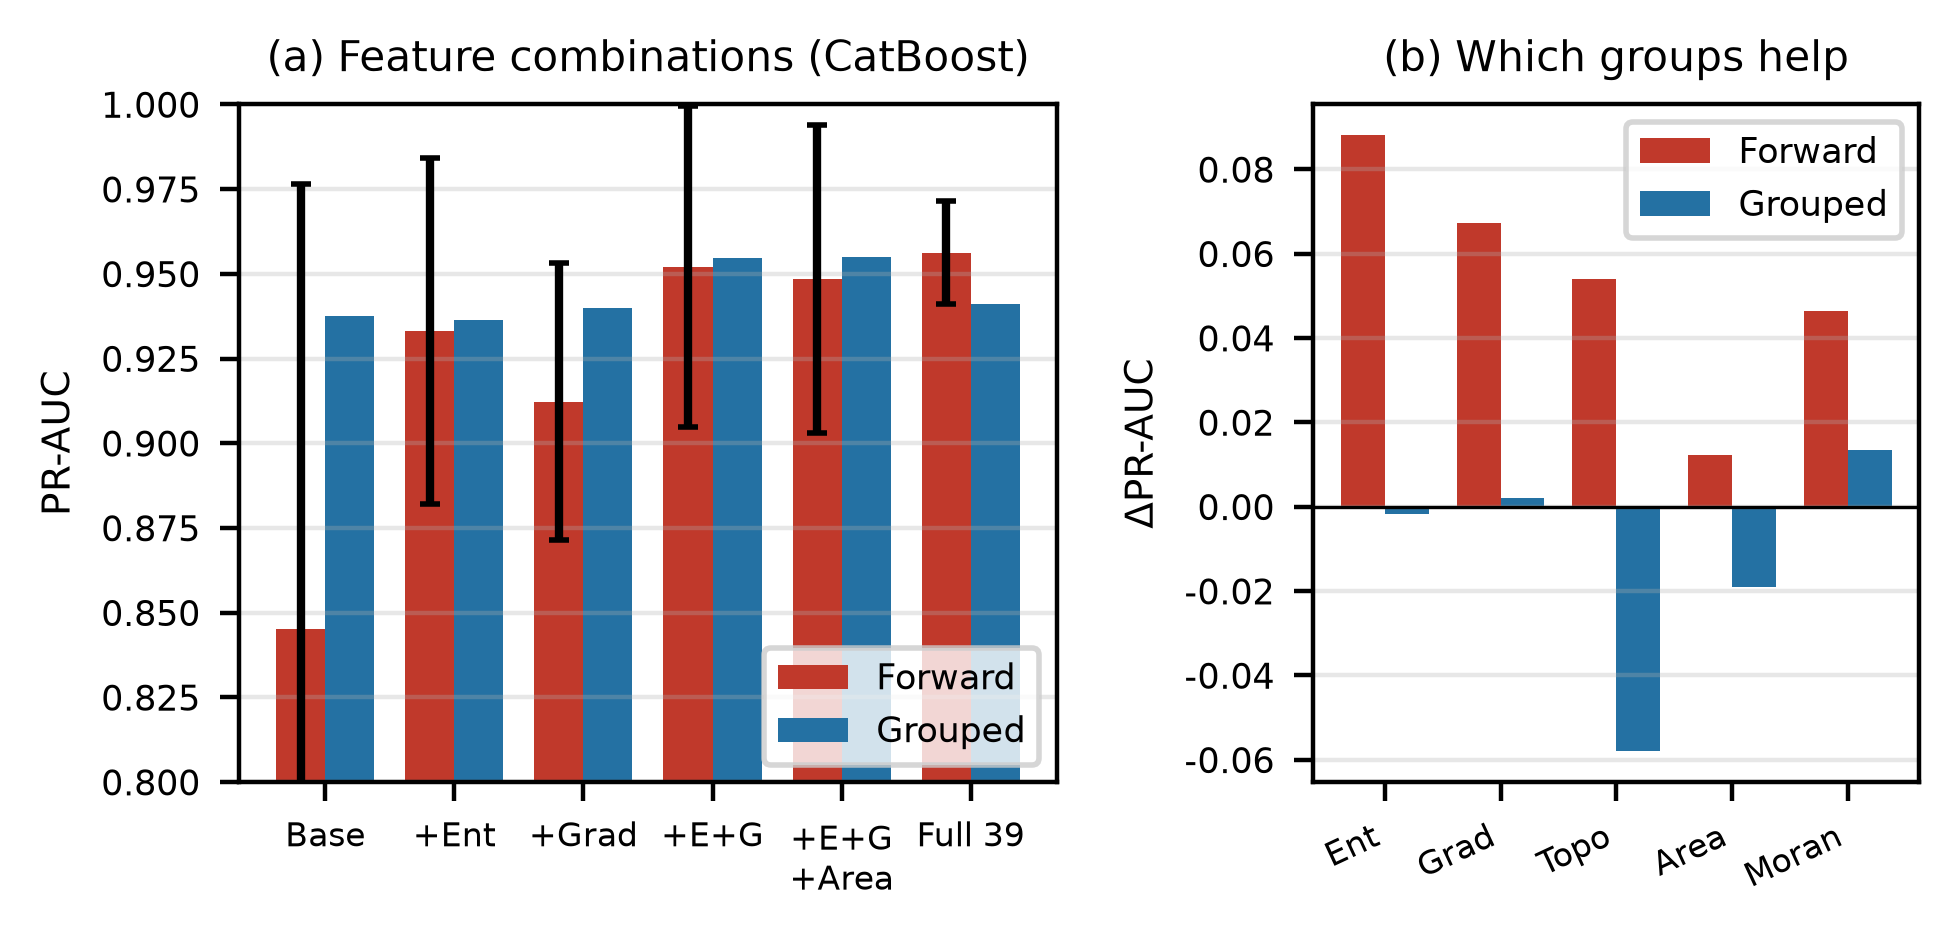
\includegraphics[width=\linewidth]{figures/fig3_ablation.png}
\caption{(a) PR-AUC for feature combinations under both protocols (CatBoost). (b) Change in PR-AUC when each descriptor group is added to the baseline; entropy and gradients help under extrapolation, topology and Moran's $I$ do not.}
\label{fig:ablation}
\end{figure}

\subsection{Control ablations}
\label{sec:controls}

Two controls test whether the gain reflects thermal-field information or merely three additional
inputs (Table~\ref{tab:controls}).

A \emph{permutation control} replaces the three descriptors with the same values shuffled across
frames. This preserves each marginal distribution while destroying any association with the frame,
so the model sees three features of realistic magnitude carrying no information. Over ten
permutations the forward-chained PR-AUC is $0.8625 \pm 0.0147$, a gain of $0.017$ over the baseline
and far below the $0.107$ obtained with the true descriptors. Three random linear projections of the
standardised field reach $0.8693 \pm 0.0226$, again well below. The gain is therefore not an effect
of adding dimensions.

A second control asks whether any three distribution statistics would do as well. Skewness,
kurtosis and the root-mean-square of the frame reach 0.931, a substantial gain of 0.086. Field-level
statistics in general, and not only the descriptors proposed here, therefore carry transferable
information. The complexity descriptors nevertheless remain significantly better: across 21 splits
(seven boundaries $\times$ three seeds) they average 0.974 against 0.947 for the moments, a paired
difference of $+0.028$ (95\% CI $[0.008, 0.051]$, $p<0.0001$), and adding the moments on top of the
descriptors changes nothing ($+0.006$, 95\% CI $[-0.006, 0.017]$, $p=0.30$). The three descriptors
thus subsume what generic moments capture, plus more.

\begin{table}[t]
\centering
\small\setlength{\tabcolsep}{4pt}
\caption{Control ablations. Each condition adds three features to the 18-dimensional baseline.
Forward chaining uses $k=20,30,40,50$ except where the multi-split column is given.
Permutation and projection controls are repeated over seeds (mean $\pm$ s.d.).}
\label{tab:controls}
\begin{tabular}{lccc}
\toprule
Condition (3 features) & Fwd (4) & Fwd (21) & Grouped \\
\midrule
Baseline (no addition)         & 0.845 & 0.888 & 0.938 \\
Permuted (null)                & $0.863 \pm 0.015$ & -- & $0.922 \pm 0.017$ \\
Random projections             & $0.869 \pm 0.023$ & -- & $0.929 \pm 0.014$ \\
Generic moments                & 0.931 & 0.947 & 0.943 \\
\textbf{Complexity}                     & \textbf{0.952} & \textbf{0.974} & \textbf{0.955} \\
Both                           & -- & 0.980 & -- \\
\bottomrule
\multicolumn{4}{p{0.95\linewidth}}{\footnotesize Generic moments are skewness, kurtosis and root-mean-square of the frame; Fwd denotes forward chaining.}
\end{tabular}
\end{table}

\subsection{Stability across seeds and boundaries}

A single split is a noisy estimate. We therefore repeat every configuration over ten random seeds and seven forward-chaining boundaries (Table~\ref{tab:multiseed}). The paired gain is positive in every model and protocol, with confidence intervals that exclude zero. For CatBoost under forward chaining the mean PR-AUC rises from 0.903 to 0.970, the paired gain is $+0.068$ with a 95\% interval of $[0.050, 0.086]$, and the standard deviation across splits falls from 0.083 to 0.029, a reduction of 65\%.

\begin{table}[t]
\centering
\small\setlength{\tabcolsep}{4pt}
\caption{Stability analysis: ten seeds $\times$ seven forward-chaining boundaries ($k=15,\dots,45$). Paired bootstrap over splits (1000 resamples).}
\label{tab:multiseed}
\small
\begin{tabular}{llcccc}
\toprule
Model & Protocol & Base & +E+G & $\Delta$ & 95\% CI \\
\midrule
\multirow{2}{*}{XGBoost}  & Grouped & $0.919\pm0.074$ & $0.943\pm0.077$ & $+0.024$ & $[0.016, 0.034]$ \\
                          & Forward & $0.903\pm0.094$ & $0.951\pm0.044$ & $+0.048$ & $[0.027, 0.070]$ \\
\multirow{2}{*}{CatBoost} & Grouped & $0.933\pm0.072$ & $0.951\pm0.078$ & $+0.018$ & $[0.011, 0.025]$ \\
                          & Forward & $0.903\pm0.083$ & $\mathbf{0.970\pm0.029}$ & $\mathbf{+0.068}$ & $[0.050, 0.086]$ \\
\multirow{2}{*}{RF} & Grouped & $0.850\pm0.041$ & $0.909\pm0.095$ & $+0.060$ & $[0.041, 0.079]$ \\
                          & Forward & $0.811\pm0.162$ & $0.903\pm0.126$ & $+0.093$ & -- \\
\bottomrule
\end{tabular}
\end{table}

Because the multiseed estimates average over seven boundaries they are higher than the single-run values in Table~\ref{tab:baseline}, which use four boundaries and one seed. The two tables answer different questions: Table~\ref{tab:multiseed} estimates the expected performance over plausible splits, whereas Table~\ref{tab:baseline} supports the comparison between models and protocols on a fixed split design.

\subsection{Separation from the substrate artefact}
\label{sec:robust}

Since 59\% of pore frames sit in layers 1 and 2, a model could score well by learning build position. We therefore repeat the analysis after removing those two layers, leaving 1513 frames and 29 pore frames. The gain does not disappear; it increases (Table~\ref{tab:robust}, Fig.~\ref{fig:robust}b). For XGBoost under forward chaining, PR-AUC rises from 0.822 to 0.954, a gain of 0.132 compared with 0.048 on the full data. The complexity descriptors therefore capture a signal that is present in the bulk of the build and is not a restatement of proximity to the substrate.

\begin{table}[t]
\centering
\small\setlength{\tabcolsep}{4pt}
\caption{Robustness checks. Left block: layers 1--2 removed (1513 frames, 29 pore frames). Right block: layer-level decisions with max aggregation.}
\label{tab:robust}
\begin{tabular}{llccc}
\toprule
Setting & Model & Base & +E+G & $\Delta$ \\
\midrule
\multirow{3}{*}{Excl.\ layers 1--2} & XGB      & 0.822 & 0.954 & $+0.132$ \\
                                     & CatBoost & 0.881 & 0.958 & $+0.077$ \\
                                     & RF       & 0.808 & 0.871 & $+0.063$ \\
\midrule
\multirow{2}{*}{Layer level}         & XGB      & 0.963 & 0.983 & $+0.020$ \\
                                     & CatBoost & 0.983 & 1.000$^{*}$ & $+0.017$ \\
\bottomrule
\multicolumn{5}{p{0.95\linewidth}}{\footnotesize $^{*}$Each test segment contains ten layers; 1.000 should not be read as a population estimate.}
\end{tabular}
\end{table}

\begin{figure}[t]
\centering
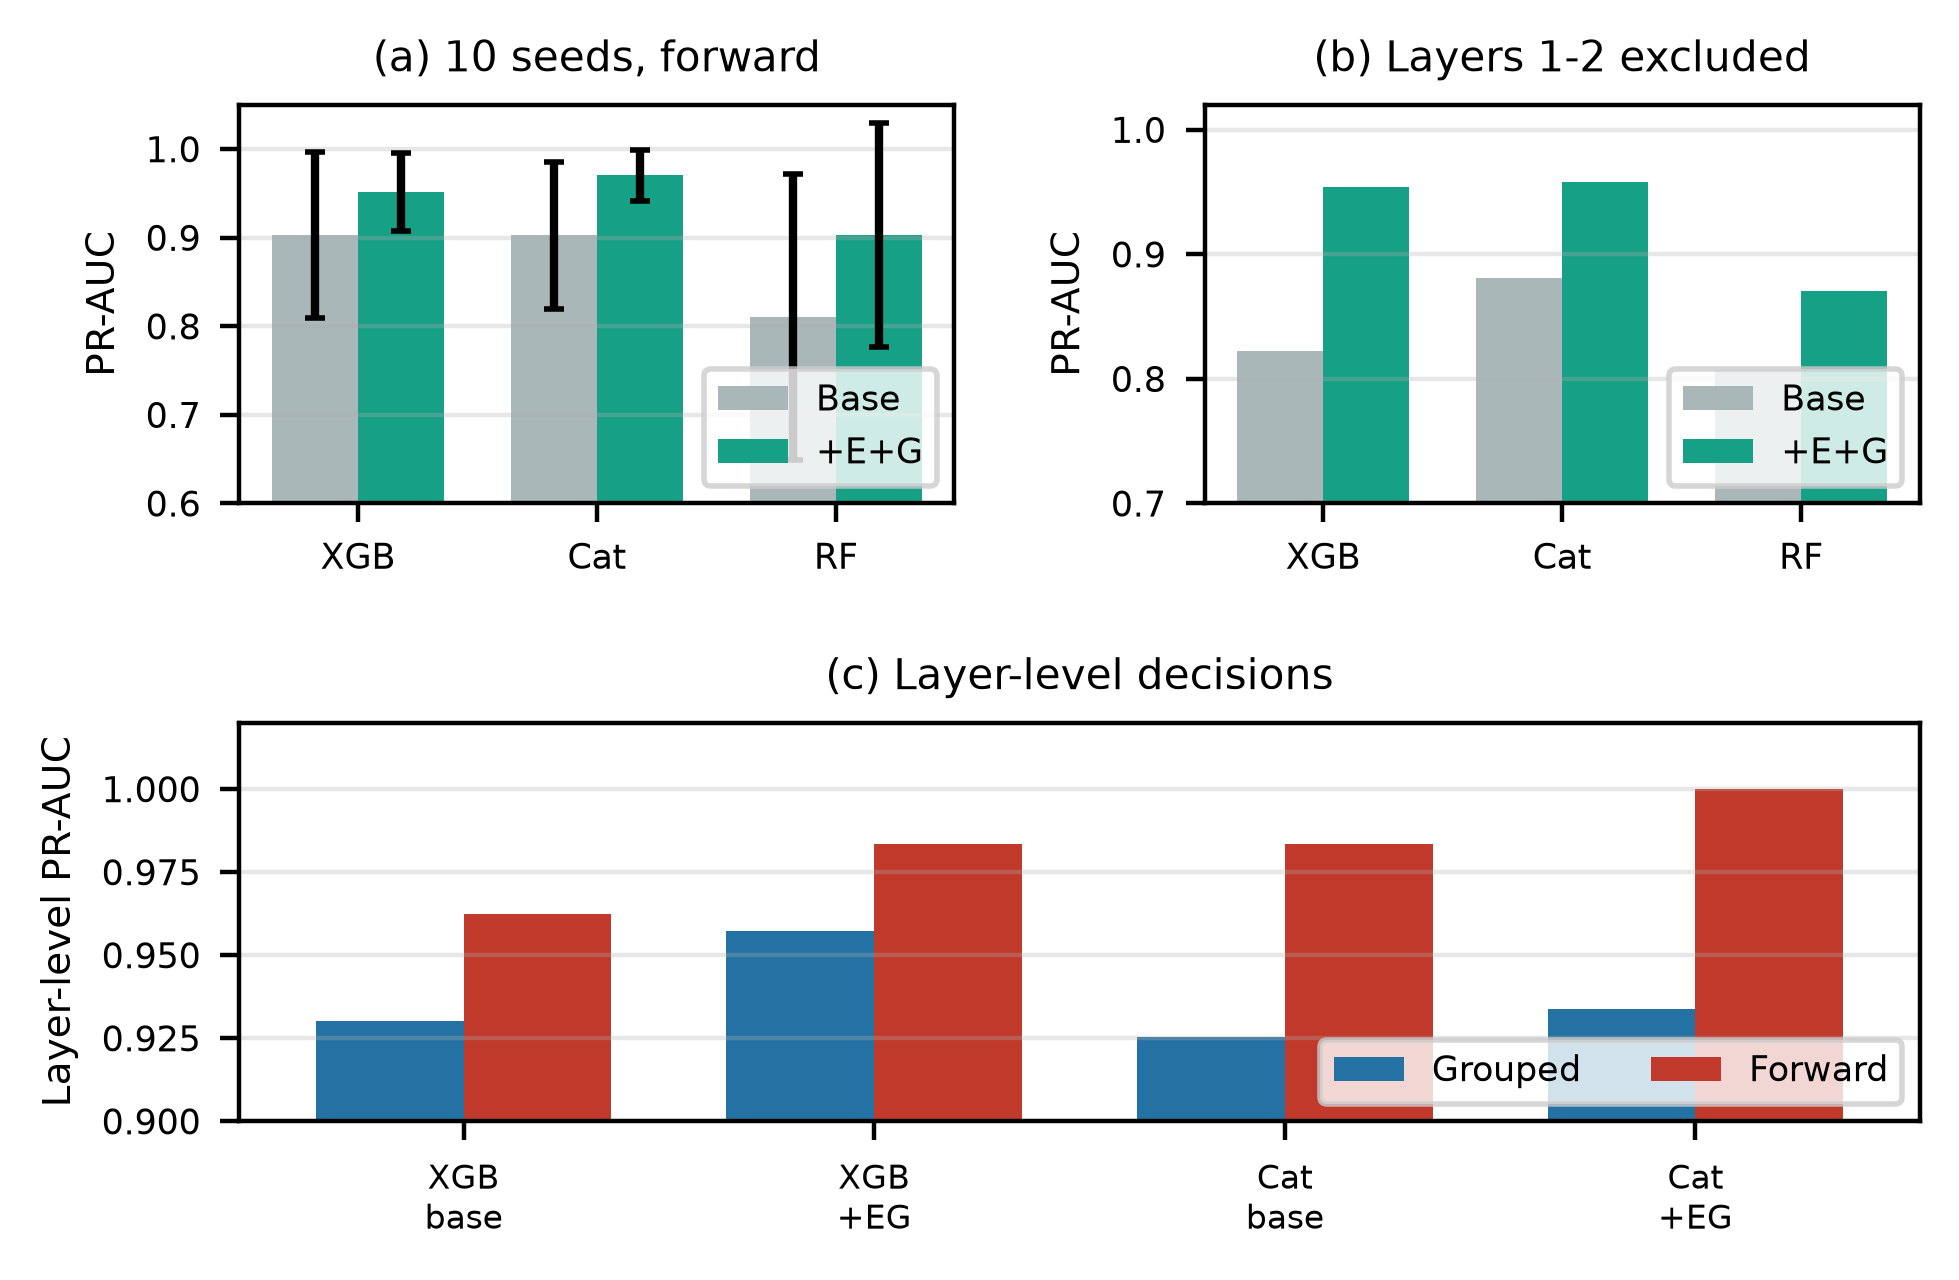
\includegraphics[width=\linewidth]{figures/fig4_robustness.png}
\caption{(a) Forward-chained PR-AUC over ten seeds for the baseline and the extended feature set. (b) The same comparison after removing layers 1--2. (c) Layer-level PR-AUC with max aggregation over frames.}
\label{fig:robust}
\end{figure}

At the layer level, where the decision unit matches the spatial resolution of the XCT labels, forward-chained PR-AUC reaches 0.983 for XGBoost. The CatBoost value of 1.000 is obtained on ten-layer test segments and is reported for completeness only.

\subsection{The same features under the literature protocol}

If the descriptors encode transferable physics, they should also perform under a random split. They do not (Table~\ref{tab:icinco}). Reproducing the protocol of \cite{ayyildizli2025}---stratified 70/30 split, SMOTE on the training portion, ten repetitions---A reimplementation of their summary-statistic descriptors reaches an F1 of 0.895 with a random forest and 0.895 with XGBoost, whereas our 21-dimensional set reaches 0.859 and 0.872. Our values sit 0.04--0.08 F1 above their reported 0.86 and 0.82; the ranking is reproduced but the absolute values are not identical, which we attribute to the eleventh descriptor being unspecified in the source and to implementation details of the resampling. The gap between feature sets is large relative to this uncertainty.

\begin{table}[t]
\centering
\small\setlength{\tabcolsep}{4pt}
\caption{Reproduction of the random-split protocol of \cite{ayyildizli2025} (70/30 stratified, SMOTE, ten repetitions).}
\footnotesize
\label{tab:icinco}
\begin{tabular}{llccccc}
\toprule
Feature set & Model & Precision & Recall & F1 & Accuracy & PR-AUC \\
\midrule
11 summary stats & Random forest & 0.828 & 0.976 & $\mathbf{0.895}$ & 0.990 & 0.922 \\
                          & XGBoost       & 0.834 & 0.967 & $\mathbf{0.895}$ & 0.990 & 0.900 \\
Our 21-dimensional set    & Random forest & 0.803 & 0.929 & 0.859 & 0.986 & 0.897 \\
                          & XGBoost       & 0.827 & 0.929 & 0.872 & 0.988 & 0.904 \\
\bottomrule
\end{tabular}
\end{table}

This result is the pivot of the paper. The descriptors do not improve interpolation; they improve extrapolation. Under a random split the model can lean on elapsed time and layer position, and adding complexity descriptors merely dilutes an already sufficient feature set. Under forward chaining those proxies extrapolate poorly, and the descriptors become the only route to the same accuracy. We return to this in Section~\ref{sec:disc}.

\subsection{From scores to decisions}

Three analyses translate the classifier into a monitoring policy.

\paragraph{Cost-sensitive operating points} When a miss costs $R$ times a false alarm, the threshold that minimises expected cost can be selected on out-of-fold predictions. Table~\ref{tab:cost} reports the resulting trade-off. At a ratio of 20:1, which is plausible for a production line where an unnecessary inspection is far cheaper than an escaping defect, recall reaches 0.95 at a precision of 0.59.

\begin{table}[t]
\centering
\small\setlength{\tabcolsep}{4pt}
\caption{Cost-sensitive operating points for CatBoost with the complexity descriptors under forward chaining.}
\label{tab:cost}
\begin{tabular}{cccc}
\toprule
Cost ratio & Recall & Precision & Norm. cost \\
\midrule
1:1   & 0.793 & 0.854 & 0.0078 \\
2:1   & 0.829 & 0.854 & 0.0054 \\
5:1   & 0.900 & 0.658 & 0.0039 \\
10:1  & 0.900 & 0.635 & 0.0031 \\
20:1  & 0.950 & 0.594 & 0.0017 \\
50:1  & 1.000 & 0.552 & 0.0003 \\
\bottomrule
\end{tabular}
\end{table}

\paragraph{Abstention} Ranking frames by confidence and abstaining on the least confident fraction removes errors disproportionately. Abstaining on 10\% of frames reduces the miss rate from 0.25 to 0.00 with the baseline features and from 0.20 to 0.00 with the complexity descriptors (Fig.~\ref{fig:decision}b). The practical reading is a two-tier policy: 90\% of frames are decided automatically with no misses, and 10\% are routed to human review.

\paragraph{Conformal prediction} Split conformal prediction on held-out layers gives empirical coverage of 0.959 at a target of 0.90 for XGBoost, with an average prediction-set size of 0.96, i.e.\ conservative coverage at almost no cost in set size. TabPFN, despite its higher PR-AUC, under-covers at 0.723, because its probabilities saturate near zero and one and the nonconformity scores become uninformative. A sharp classifier can thus be a poor basis for calibrated decisions.

\begin{figure}[t]
\centering
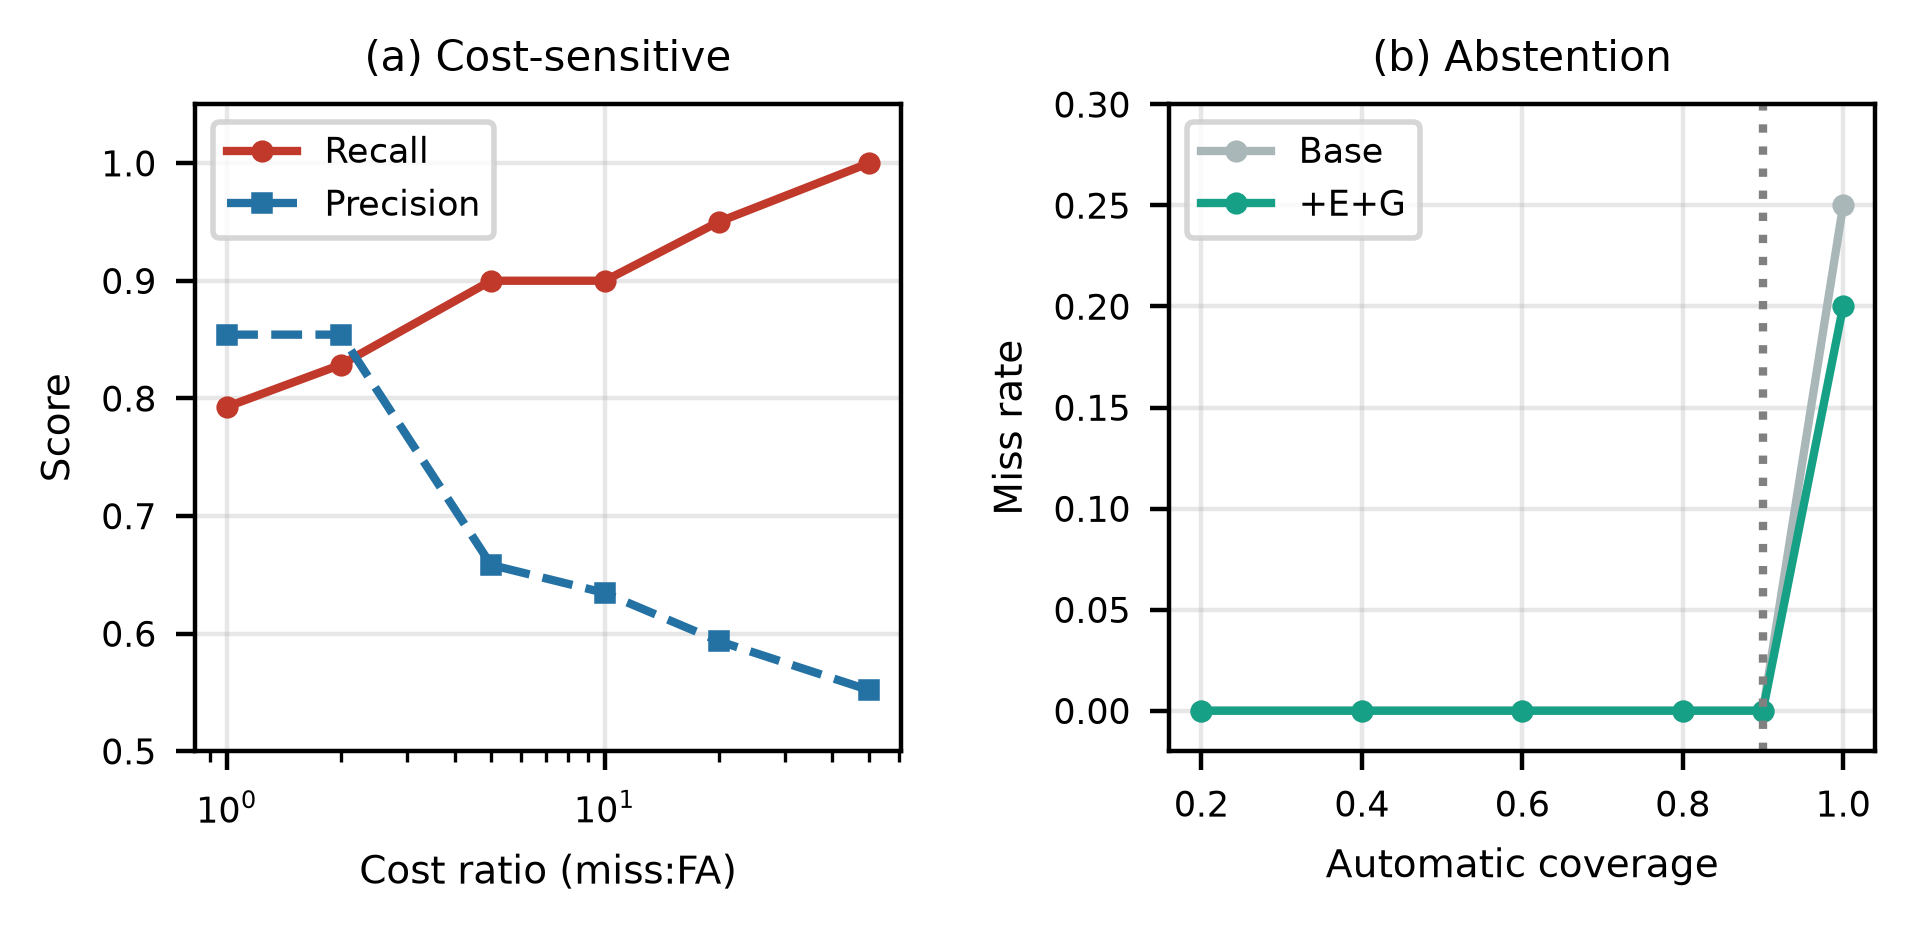
\includegraphics[width=0.92\linewidth]{figures/fig6_decision.png}
\caption{(a) Cost-sensitive operating points. (b) Miss rate as a function of the fraction of frames decided automatically; abstaining on the least confident 10\% eliminates misses.}
\label{fig:decision}
\end{figure}

\subsection{What the model has learned}
\label{sec:shap}

SHAP values \cite{lundberg2017} for XGBoost on the full 21-dimensional set rank histogram entropy first (mean $|$SHAP$|$ 2.59), ahead of the temperature standard deviation (2.08) and the mean gradient (1.74). Peak temperature ranks eleventh with 0.27, roughly one tenth of the entropy contribution. Removing layers 1 and 2 strengthens rather than weakens this ordering: entropy rises to 4.46 while peak temperature stays outside the top ten (Fig.~\ref{fig:shap}a).

\begin{figure}[t]
\centering
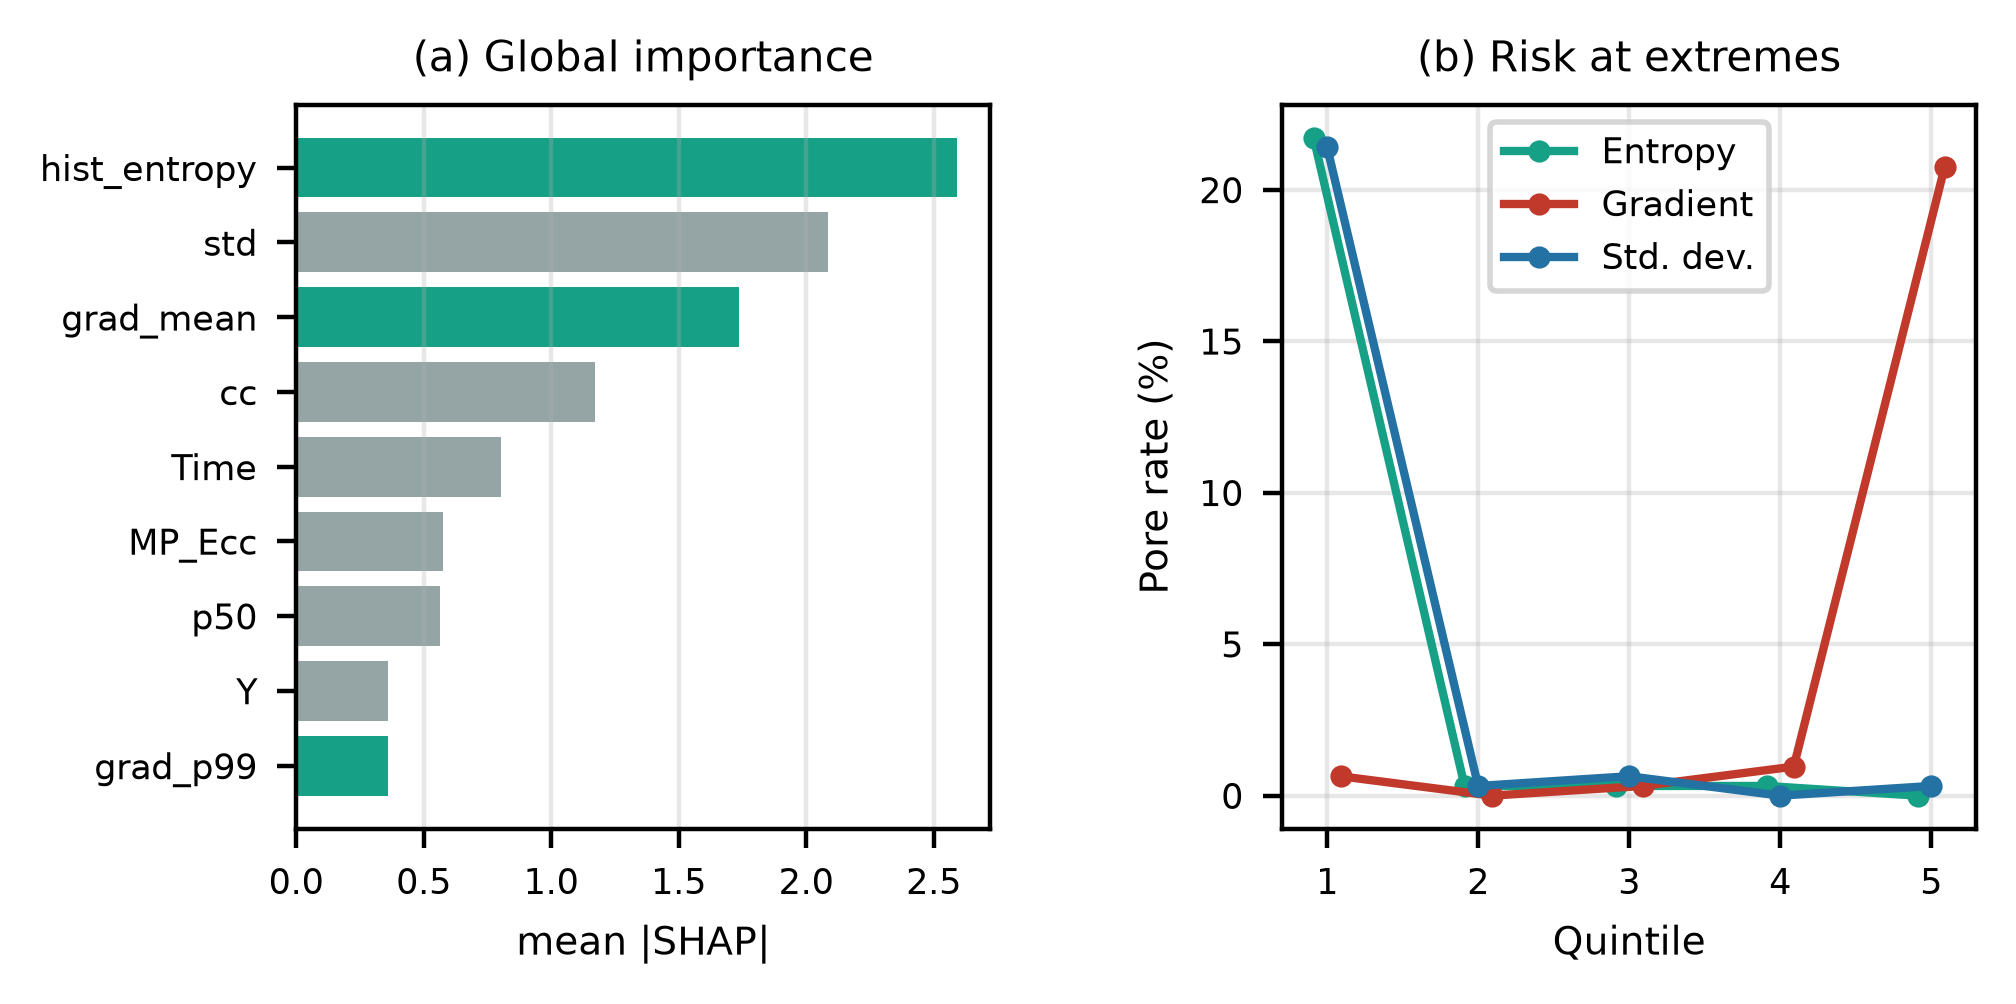
\includegraphics[width=0.95\linewidth]{figures/fig5_shap.png}
\caption{(a) Global feature importance by mean absolute SHAP value. (b) Pore rate as a function of feature quintile: risk concentrates at low entropy, low standard deviation and high gradient.}
\label{fig:shap}
\end{figure}

The shape of the dependence is informative (Fig.~\ref{fig:shap}b). Frames in the lowest quintile of entropy have a pore rate of 21.7\%, against 0.3\% or less in the other quintiles; the lowest quintile of standard deviation behaves the same way (21.4\% against at most 0.6\%); and frames in the highest quintile of mean gradient reach 20.8\% against at most 1.0\% elsewhere. After removing layers 1--2 the same pattern persists at lower absolute rates (9.6\%, 8.6\% and 8.3\% respectively). The lowest quintile alone contains 68 of the 71 pore frames while the remaining four hold one, one, one and zero; the shape of the dependence is therefore well determined, but its precise rates are not.

The three descriptors describe a single physical configuration: a melt pool whose interior is comparatively uniform while its boundary is sharp. That is what an under-energised deposit looks like when the absorbed energy is insufficient to remelt the previous layer and the pool stays shallow, so the surrounding metal remains cool and the interface stays steep. A well-formed pool spreads a broad, smoothly varying high-temperature zone, which raises entropy and lowers the peak gradient. The statistical importance of entropy over peak temperature is therefore consistent with the lack-of-fusion mechanism that dominates this specimen.

\section{Discussion}
\label{sec:disc}

\paragraph{Why the protocol changes the answer} Under grouped cross-validation, each fold contains layers drawn from across the build, so a model can associate particular values of elapsed time or height with the pore state in its own training set. Forward chaining removes that route: the test layers lie beyond every training layer, and any feature that merely indexes position must be extrapolated, which it cannot be. Features that describe the thermal state itself continue to transfer. The asymmetry between the two protocols in Table~\ref{tab:groups} is therefore a direct measurement of how much of a feature's apparent value is positional.

\paragraph{Why the deep model does not close the gap} A convolutional network operating on the raw field reaches 0.777 under grouped cross-validation and 0.688 under forward chaining, below every tabular baseline, and its performance depends strongly on the stopping criterion: with a fixed budget of 25 epochs and no early stopping the figures fall to 0.537 and 0.505. With between 538 and 1326 training frames and 51 to 66 positives depending on the split, the network must learn both a representation and a decision boundary from very few examples, and it does so unstably. The descriptors supply the representation in closed form, which is consistent with the small-data findings reported for tabular foundation models \cite{hollmann2025}.

\paragraph{Practical implications} The cost-sensitive and abstention analyses give a deployment recipe that does not depend on the absolute probability scale. A plant that accepts one false alarm per true detection sets a low threshold and inspects liberally; a plant that cannot afford stoppages sets a high threshold and accepts misses; both can read their operating point from Table~\ref{tab:cost}. The abstention result is the more actionable: routing the least confident decile to a human removes every miss in our test segments at a 10\% review burden.

\paragraph{What this changes for reported benchmarks} Headline accuracies above 0.98 on this dataset are reproducible, but they are compatible with a model that has learned little beyond process position. We recommend that future work report PR-AUC or the area under the precision--recall curve together with a forward-chaining split, and that accuracy be reported only alongside a trivial baseline.

\section{Limitations}

The study rests on a single geometry, a single alloy and a single build. Our extrapolation protocol moves along the build direction within that build, which is a necessary but weaker test than transfer to a new part. The dataset authors themselves examined transfer to cylinders but reported no quantitative error \cite{guo2023}, and we could not repeat that experiment without the corresponding data. Any claim of generalisation should therefore be read as generalisation across layers and process states, not across geometries.

The positive class is small. Twenty-nine pore frames remain after removing layers 1--2, and each forward-chaining test segment contains between four and seven. Confidence intervals are correspondingly wide, and the layer-level value of 1.000 for CatBoost reflects ten-layer test sets rather than population performance.

The convolutional baseline was trained with a single seed per split and its stopping epoch chosen on validation layers. A fixed-epoch variant performs substantially worse (0.537 grouped, 0.505 forward), so the deep-model comparison should be read as evidence of instability at this sample size rather than as a precise benchmark.

Finally, the thermal imagery alone carries limited signal for sub-millimetre pores, a limitation noted for hybrid DED monitoring \cite{farea2025}. Fusion with acoustic or optical sensing is the natural extension and lies outside the scope of a single-modality study.

\section{Conclusions}

We re-examined porosity prediction from melt-pool pyrometry on a public LENS Ti--6Al--4V dataset, asking which conclusions survive when evaluation respects the build order.

Three findings follow. First, protocol choice dominates model choice: the four strongest tabular classifiers span only 0.03 PR-AUC under grouped cross-validation, and under forward chaining their ordering changes while the top pair remains statistically indistinguishable ($p=0.80$). Accuracy stays near 0.98 throughout and carries no information about generalisation.

Second, three physically interpretable descriptors of thermal-field complexity---histogram entropy and two gradient statistics---raise forward-chained PR-AUC from 0.903 to 0.970 for CatBoost over ten seeds and seven boundaries, cut the split-to-split standard deviation by 65\%, and account for 96\% of the gain available from a 21-dimensional spatial feature set. Two controls separate information from dimensionality: permuted descriptors gain only 0.017, while generic distribution moments gain 0.086 but stay 0.028 behind ($p<0.0001$). The gain survives removal of the substrate-interface layers that contain most pore frames, where it grows to 0.132 for XGBoost.

Third, the descriptors help only under extrapolation. Under the random split used in earlier work on this dataset they are inferior to conventional summary statistics (F1 0.872 against 0.895). The asymmetry is the point: complexity descriptors encode physics that transfers, and interpolation-based evaluation hides exactly that property.

SHAP analysis places the risk at low entropy, low variance and high gradient, a signature of under-energised, shallow melt pools whose surroundings stay cool and whose boundary stays steep. Combined with cost-sensitive thresholds and a 10\% abstention policy that eliminates misses, these results offer a route from thermal monitoring to a defensible quality decision.

\section*{CRediT authorship contribution statement}

\textbf{First Author:} Conceptualization, Methodology, Software, Formal analysis, Writing -- original draft. \textbf{Second Author:} Data curation, Validation, Visualization. \textbf{Third Author:} Supervision, Writing -- review \& editing, Funding acquisition.

\section*{Declaration of competing interest}

The authors declare that they have no known competing financial interests or personal relationships that could have appeared to influence the work reported in this paper.

\section*{Data availability}

The dataset analysed in this study is publicly available at Harvard Dataverse, DOI 10.7910/DVN/BWHYEH. Analysis code and derived result tables are available at \url{https://github.com/WangAnChuan/Thermal-field-complexity-descriptors-for-porosity-prediction-in-LENS-Ti-6Al-4V}.

\bibliographystyle{elsarticle-num}
\bibliography{refs}

\end{document}
